%auto-ignore
%      this ensures the arxiv doesn't try to start TeXing here.
%!TEX root = super_lattice_models_draft.tex
%      prev line helps TeXShop do the right thing



%%%%%%%%%%%%%%%%%%%%%%%
\section{Super pivotal state sums and tensor networks} \label{state_sums}
%%%%%%%%%%%%%%%%%%%%%%%

In this section we describe a version of the Turaev-Viro-Barrett-Westbury (TVBW) state sum \cite{Turaev1992,Barrett1996}
for super pivotal fusion categories 
and a tensor network for the ground state wave function of the Hamiltonian constructed in Section \ref{Super_pivotal_Hamiltonian}.
Related 
work was presented in~\cite{bhardwaj2016}, 
see also \cite{Bultinck2017}.
We first review the TVBW construction for bosonic spherical fusion categories. 
We then show how to write the state-sum as a tensor contraction on a tensor 
network.
Next we detail the modifications needed for the fermionic versions of the state sum and tensor network.
Lastly we use the state sum to write down an explicit wave function for the ground ground state of \eqref{ham}.

\medskip

Before we begin, we need to establish some terminology regarding cell and handle decompositions. 
Recall that a handle decomposition for a 
3-manifold $M$ is built from a series of $k$-handles, with $k=0,1,2,3$, each of which is identified with $D^k\times D^{3-k}$. 
Handle decompositions can be obtained from cell decompositions by thickening each $k$-cell into a $k$-handle.
Conversely, each handle decomposition determines a cell decomposition by taking the cores of the handles.
(See Section \ref{standardized_handles} for more details.)
We will often refer to a $k$-cell and its associated $k$-handle with the same letter, since
it will be convenient for us to be able to describe things in terms of both handle decompositions 
and their corresponding cell decompositions. 
We call $S^{k-1} \times D^{3-k}$ the attaching region (or attaching boundary) of the $k$-handle,
and $D^k\times S^{3-k-1}$ the non-attaching boundary.
The attaching map of a $k$-handle is a homeomorphism from the attaching region to 
a submanifold of the boundary of the union of the lower-dimensional handles.
The topology of $M$ is encoded by the various attaching maps.
The different types of $k$-handles are illustrated in Figure 
\ref{HandleDecompFig}.

\begin{figure}
\begin{center}
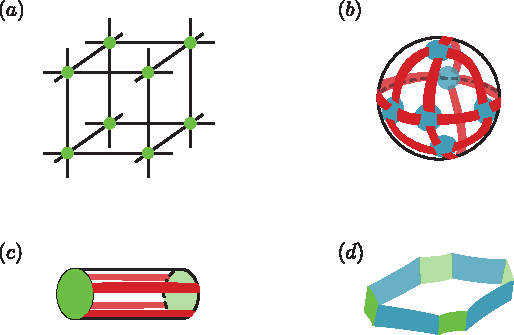
\includegraphics[scale = 1]{HandleDecompFig.pdf}
\end{center}
\caption{\label{HandleDecompFig}%
The handles corresponding to a standard cubic cell decomposition (a).
The 0-, 1- and 2-handles are shown in (b), (c) and (d), with colors green, blue and red.
In (b) the blue disks on the 0-handle indicate where the 1-handles attach to the 0-handle, and the red rectangles
indicate where the 2-handles attach to the 0-handle.
In (c) the green disks indicate where the 0-handles attach to the 1-handle and the red rectangles indicate where the 2-handles attach to the 1-handle.
Similarly, in (d) the blue and green rectangles indicate where the 2-handles attach to the 0- and 1-handles.
We have omitted the 3-handles from the figure.}
\end{figure} 


%%%%%%%%%%%%%%%%%%%%
\subsection{Bosonic TVBW state sum}
%%%%%%%%%%%%%%%%%%%%


%%%%%%%%%%%%%%%%%%%%%%%
\subsubsection{Definition of the state sum}
%%%%%%%%%%%%%%%%%%%%%%%

Our first task is to describe the TVBW (bosonic) state sum.
The original references are \cite{Turaev1992,Barrett1996}.
We will use the form for a general cell/handle decomposition, as described in \cite{Walker2006}.

Let $M$ be a closed oriented 3-manifold equipped with a handle decomposition $\mch$.
Choose auxiliary orientations of the 1- and 2-cells of the cell decomposition corresponding to $\mch$.
Let $\mch_i$ denote the set of $i$-handles ($i = 0,1,2,3$).
The state sum has the form
\be \label{bos_tv_sum}
	Z(M) = \sum_{\beta\in\mcl(\mch)}
		\prod_{c\in\mch_3} \mcd^{-2}
		\prod_{f\in\mch_2} d(f, \beta)
		\prod_{e\in\mch_1} \widetilde\Theta(e, \beta)^{-1}
		\prod_{v\in\mch_0} \text{Link}(v, \beta) .
\ee
The next few paragraphs define the notation used in \eqref{bos_tv_sum}.

We use the 2-cell orientations to define an oriented graph (unlabeled string net) on the boundary of each 0-, 1- and 2-handle,
as shown in Figure \ref{TwoHandleToGraph}.
String-net graphs are assigned to the $k$-handles as follows:
\begin{figure}
\begin{center}
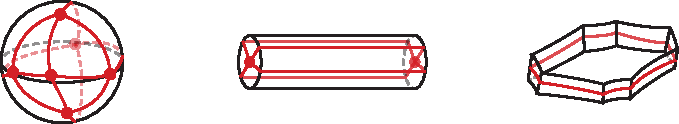
\includegraphics[scale = 1]{NetsonHandles.pdf}
\end{center}
\caption{\label{TwoHandleToGraph}%
Graphs on the boundaries of 0-, 1- and 2-handles, in the case of a cubic cell decomposition.
Compare Figure \ref{HandleDecompFig}.}
\end{figure} 
\begin{itemize}
\item On 2-handles, the graph is a single loop along the core of the attaching annulus of a 2-handle.
The orientation of the loop is determined by the orientation of the 2-cell. 
\item On 1-handles, the graph is a generalized $\Theta$ graph, which we will call a $\widetilde\Theta$ graph.
The graph has one edge for each 2-handle adjacent to the 1-handle.
The middle part of each edge of the graph corresponds to where the cores of the 2-handles meet the boundary of the 1-handle.
The two vertices of the graph are on the two attaching disks of the 1-handle.
The edges are oriented opposite to the orientations used in the 2-handle loops above.
\item On each 0-handle, the graph is determined by the pattern of 2- and 1-handles adjacent to the 0-handle.
The graph has one edge for each adjacent 2-handle and one vertex for each adjacent 1-handle.
The orientations of the edges are opposite to the orientations of the 2-handle loops.
We denote this graph $\text{Link}(v)$.
\end{itemize}

\begin{figure}
\centering
\begin{align}
\nonumber
\CellDecompNearOneHandle \quad \quad \quad \quad \quad \OneHandlePrime 
\end{align}
\caption{\label{OneHandlePrime}
On the left, we have an illustration of four 2-cells meeting a 1-cell.
For clarity we have put a small gap between the 1-cell and the four 2-cells.
On the right we have the corresponding 1-handle and a particular labeling. 
We have denoted the corresponding attaching disks by `i' for initial, and `t' for terminal. 
}
\end{figure}

Recall that we have an orientation of each 1-cell.
This allows us to distinguish an ``initial" and ``terminal" attaching disk for each 1-handle; see Figure \ref{OneHandlePrime}.
On the initial disk we see a graph with a single vertex in the interior of the disk and $k$ edges connecting the central vertex
to the boundary of the disk (where $k$ is the number of 2-handles which cross the 1-handle).
For each labeling $\ell$ of these edges by simple objects in $\sob(\mcc)$, we have an associated vector space $V(\ell)$.
For example, in the case of Figure \ref{OneHandlePrime} the vector space is isomorphic to $V^{ab^*c^*d}$.
Let $B(\ell)$ be some chosen basis of this vector space.
For each 1-handle $e$ define $B(e)$ to be the union over all labelings $\ell$ of $B(\ell)$,
and also define $V(e)$ to be the direct sum of all the vector spaces $V(\ell)$.

We define the set of all labelings $\mcl(\mch)$ to be the product over all 1-handles $e$ of the basis sets $B(e)$.
In other words, we choose (independently, without any compatibility constraints) a labeling by simple objects of the edges of each initial
disk graph, then choose a basis vector for each associated vector space.

We also associate a vector space $V^*(\ell)$ to the terminal disk of each labeled 1-handle.
In the example, this is isomorphic to $V^{d^*cba^*}$.
There is a nondegenerate bilinear pairing between $V(\ell)$ and $V^*(\ell)$, 
given by evaluating the labeled string net on the boundary of the 1-handle (which is a 2-sphere).
We will choose a basis of $V^*(\ell)$ such that the pairing matrix is diagonal.
(It is sometimes convenient to not insist that the diagonal entries be $\delta_{ij}$.)
We also define $V^*(e)$ to be the direct sum (over all labelings $\ell$) of $V^*(\ell)$.

We are now ready to define the weights appearing in the state-sum $Z(M)$. 
Let $\beta\in\mcl(\mch)$ and let $f$ be a 2-handle.
The labeling $\beta$ associates a simple object to each intersection of $f$ with a 1-handle.
If these simple objects are not all the same, we define $d(f, \beta) = 0$.
If they are all equal to the same simple object $a\in\sob(\mcc)$, we define the weight $d(f, \beta)$
appearing in \eqref{bos_tv_sum} by $d(f,\beta) = d_a$.

Let $e$ be a 1-handle.
The labeling $\beta$ associates a basis vector $\mu$ to the initial disk of $e$.
Define $\widetilde\Theta(e, \beta)$ to be the value of the bilinear pairing evaluated on $\mu^*$ and $\mu$.
Diagrammatically, $\widetilde\Theta(e, \beta)$ is found by connecting the open strings in $V(\ell)$ to their dual counterparts in $V^*(\ell)$ and evaluating 
the resulting diagram.
Continuing with our example in Figure \ref{OneHandlePrime}, 
we have 
\be \label{four_banana}
\widetilde \Theta (e, \beta) =  \Bananafourmu.
\ee

\begin{figure}
\centering
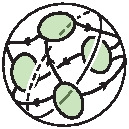
\includegraphics{TetSphereColored.pdf}
\caption{ \label{TetSphere_Fig} 
An example of the surface of a 0-handle on which four 1-handles are attached to. 
The attaching regions for the 1-handles are marked in green. The coloring $\beta$ assigns 
objects to the oriented strands and fusion space basis vectors to the green regions.
}
\end{figure}

Let $v$ be a 0-handle.
The labeling $\beta$ determines a labeling of the graph $\text{Link}(v)$ as follows.
Near each vertex of $\text{Link}(v)$ we place the basis element $\mu^* \in V^*(e)$ (or $\mu \in V(e)$) assigned by $\beta$ to the 
corresponding 1-handle if $v$ is attached to the initial (terminal) end of the 1-handle.
If these vertex labels are incompatible along edges of $\text{Link}(v)$, we define $\text{Link}(v, \beta) = 0$.
If they are all compatible then we define $\text{Link}(v, \beta)$ to be the evaluation of the resulting labeled graph (string net).
For cell decompositions dual to a triangulation, 
the labeled graph is a tetrahedral string net on a sphere.
This is illustrated in Figure \ref{TetSphere_Fig}, which shows an example 0-handle on which 
four 1-handles terminate. 

This completes the definition of the state sum.

\medskip

It follows from Section 8.2 of \cite{Walker2006} that the state sum computes $Z(M)$, independently of the choice of handle decomposition
and choice of orientations of 1- and 2-cells.

\medskip

If $M$ has non-empty boundary,
then we choose the cell decomposition so that $\bd M$ lies in the union of the 2-skeleton (union of 0-1, 1- and 2-cells).
(An alternative choice would be to require that $\bd M$ is transverse to the 2-skeleton.
The two conventions each have strengths and weaknesses.)

The 0- and 1-cells on $\bd M$ will do double duty as the underlying graph of a string net on $\bd M$.
Choose an orientation of each 1-cell on $\bd M$.
(This is analogous to choosing an orientation of the boundary of a 2-cell in the interior of $M$.)
Choose a labeling of these oriented edges by simple objects in $\sob(\mcc)$.
For each vertex (0-cell) on $\bd M$, choose an element of the appropriate disk vector space.

We now have a labeled string net $g$ on $\bd M$.
The state sum will evaluate the path integral $Z(M)(g)$ 
(i.e.\ the path integral of $M$ with boundary condition given by $g$).
The labelings and weights are defined as before, except that some of the labels are already determined by the string net $g$ on the boundary.


%%%%%%%%%%%%%%%%%%%%%%%%%
\subsubsection{The state sum as a tensor network}
%%%%%%%%%%%%%%%%%%%%%%%%%

Our goal in this subsection is to reinterpret \eqref{bos_tv_sum} as a tensor network.
We will first discuss that case when $M$ is closed, then consider the case when $\bd M$ is non-empty.

\medskip

If we (temporarily) ignore the factors of $d(f, \beta)$ and $\mcd^{-2}$ in \eqref{bos_tv_sum}, 
it is easily seen to compute the contraction of a tensor network.
The underlying graph of the tensor network is the union of 0- and 1-cells of the cell decomposition.
The vector space associated to each edge $e$ is $V(e)$ as defined above.
The matrix elements of the tensor associated to a 0-cell $v$ are the numbers $\text{Link}(v, \beta)$ defined above.
The factors of $\widetilde\Theta(e, \beta)^{-1}$ arise from the pairing of dual tensor indices.

To incorporate the factors of $d(f, \beta)$ and $\mcd^{-2}$, we make some ad hoc choices.
We consider ``dressed" 
0-handle weights that incorporate the factors of $d(f,\beta)$ and $\mcd^{-2}$ for certain adjacent 2- and 3-cells.
For each 2-handle $f$ we choose an adjacent 0-handle $v_f$.
For a 0-handle $v$ we modify the associated weight ${\text{Link}}(v,\beta)$ by multiplying factors of $d(f,\beta)$ for each 2-handle $f$ such that $v = v_f$.
Similarly, for each 3-handle we choose an adjacent 0-handle and multiply the associated weight by $\mcd^{-2}$.
Denoting the modified 0-handle weights by $\widetilde{\rm Link}(v,\beta)$, 
we define the 0-handle tensors $T_v$ as follows.
Let $e_1, \ldots, e_k$ be the 1-handles adjacent to the 0-handle $v$.
Let 
\begin{align}
\label{0_handleVectorspaces}
V_i = \begin{cases}
V(e_i) & \text{if $v$ is adjacent to the terminal end of $e_i$}\\
V^*(e_i) & \text{ if $v$ is adjacent to the initial end of $e_i$}.\\
\end{cases}
\end{align}
We define
\be
	T_v \in V^*_1\tp\cdots\tp V^*_k
\ee
by
\be
\label{vertex_tensor}
	T_v(w_1\tp\cdots\tp w_k) = \widetilde{\text{Link}}(v, w_1\tp\cdots\tp w_k),
\ee
where $w_i\in V_i$.
In other words, $T_v$ evaluates the link graph with labels determined by $w_1,\ldots,w_k$ and multiplied by the factors of $d(f,\beta)$ and $\mcd^{-2}$ as described above.
To obtain the partition function, we trace out the tensor product of all the 0-handle tensors constructed in this way.
Because the vector space associated to the region on a $0$-handle attached to the 
terminal end of a 1-handle $e$ is dual to the vector space associated to the corresponding region on the 
0-handle attached to the initial end of $e$, there are precisely as many dual vectors as vectors in the tensor product, and 
contracting each vector with its associated dual vector computes the complex number $Z(M)$. 
That is, we have 
\be Z(M) = \tr \left(\bigotimes_{v\in \mch_0} T_v\right),\ee
where the trace $\tr$ denotes the tensor contraction.
It is easy to see that this tensor network gives the same state sum as \eqref{bos_tv_sum} and 
is independent of the way we assign factors of $d(f,\beta)$ and $\mcd^{-2}$ to the 
vertex tensors. 

\medskip

In the case where $\partial M \neq \emptyset$, we define the 0-handle tensors $T_v$ as before,
but in this case some of the legs of the tensors are unpaired (not contracted).
Specifically, there is one unpaired leg for each 0-cell on $\bd M$.
If $W_1, \ldots, W_n$ are the vector spaces associated to the boundary 0-cells, we have
\be \label{trace_pM_nonempty}
	Z(M) = \tr \left( \bigotimes_{v\in \mch_0} T_v \right) \in W_1^*\tp\cdots\tp W_n^* .
\ee
Each string net on $\bd M$ (i.e. each labeling of 0- and 1-cells as described above)
determines an element of $W_1\tp\cdots\tp W_n$ (the vertex labels).
By evaluating \eqref{trace_pM_nonempty} on this element we obtain the amplitude of the wave function for the string net.


%%%%%%%%%%%%%%%%%
\subsubsection{Standardization procedures} \label{bosonic_standardization} 
%%%%%%%%%%%%%%%%%

The above tensor network construction is irregular, in the sense that (potentially) every edge vector space is different 
and every 0-handle tensor is different.
There are several standardization procedures that reduce this irregularity. 

One standardization procedure is to start with a cell decomposition that is dual to a triangulation.
This ensures that there are exactly three 2-handles meeting each edge, and that the vertex graphs $\text{Link}(v,\beta)$ are all tetrahedral.
However, this still leaves us with several different types of edge vector spaces and vertex tensors.
For example, depending on the choice of 1- and 2-cell orientations, there will be eight possible vector spaces associated to 1-handles,
corresponding to $V^{abc}$, $V^{ab^*c}$, $V^{a^*b^*c^*}$, etc.
(Note that if all Frobenius-Schur indicators are equal to 1, then we can ignore these distinctions.)
Similarly, there will be many different tetrahedral vertex tensors, depending on the orientations of the edges of the tetrahedral graph.

We can further standardize the tensor network by choosing a global ordering of the 3-cells of the handle decomposition.
(This is equivalent to a global ordering of the vertices of the dual triangulation.)
We then choose 2-cell orientations so that the the orientation of a 2-cell together with a normal vector pointing toward the higher-ordered of the two
adjacent 3-cells agrees with the orientation of $M$.
We can now choose 1-cell orientations so that the graph on the initial disk of each 1-handle has a trivalent vertex with two
outgoing and one incoming edge.
With these orientation choices, we have, for every 1-handle $e$,
\be
	V(e) = \bigoplus_{a,b,c\in\sob(\mcc)} V^{abc^*} .
\ee
Furthermore, all of the tetrahedral graphs have the same pattern of edge orientations, so all of the 0-handle tensors
in the tensor network are of the same form. 

However, it is not always convenient to choose a global ordering.
For example, our main application is a tensor network associated to $Y\times I$.
If $Y$ is a torus, we might hope that the network has translational symmetry, but this is not compatible with the global ordering trick.
For this reason, in what follows we will work with a cell decomposition dual to a triangulation, but we will not employ the global ordering trick.

We will find it useful to employ a standardization 
procedure in which all fusion spaces in the string nets assigned to the 0-handles 
assume the ``pitchfork'' form introduced 
in our treatment of the Hamiltonian. 
(These vertices are all trivalent since we are now 
assuming a cell decomposition dual to a triangulation.)
In this convention, the $T_v$ tensor weights are all computed by the evaluation of tetrahedral diagrams:
\begin{align} 
\label{Bosonic_tet}
	T_v(\alpha \tp \beta \tp \gamma \tp \delta) = {\rm Tet}(v,\alpha \tp \beta \tp \gamma \tp \delta) = \TetrahedronPrime , 
\end{align}
where we have defined the tensor weight by its evaluation of the picture on the right with 
$\alpha \in \bigoplus_{abc} V^{abc}$, $\beta \in \bigoplus_{abc} V^{a^* bc}$, $\gamma \in \bigoplus_{abc} V^{a^* b^* c^*}$, and $ \delta \in \bigoplus_{abc} V^{a^* b c^*}$.
The pitchforkization procedure does not entirely fix the form of the $T_v$ tensors above, 
since the tetrahedral nets associated with each 0-handle will in general have different 
edge orientations.  
Since there are $2^6 = 64$ possible choices of edge orientations near a 0-handle, there will be 64 
different types of $T_v$ tensors, given by the appropriate diagram evaluation with $\alpha,\beta,\gamma,\delta$ chosen from the appropriate fusion spaces.%
\footnote{Not all these $64$ tetrahedra are independent however, as 
some of them can be transformed into one another by using the pivotal and spherical structure of the input category.}

In this procedure, we choose standardizations (pitchforkizations) at each 0-handle independently.
This means that the two ends of each 1-handle are standardized independently 
of each other, and the pairing induced from the $\widetilde\Theta$ graph on the 1-handle 
\eqref{four_banana}
will not necessarily agree with the standard pairing \eqref{reflection_pairing_defn}.
Instead, the 1-handle pairing and the standard pairing will be 
related by a pivot operation $P_e=P^{l_e}$ for $l_e = 0,1,2$, where $P$ is the pivot defined in \eqref{Pitchfork_pivot}.
We define $P_e$ to rotate diagrams counterclockwise relative to the orientation of $e$. 
If $l_e \neq 0$, then the 
pitchforks at the
initial and terminal vertices of $e$ are twisted by $2\pi l_e / 3$ relative to 
one another, and this twisting data needs to be incorporated into the 1-handles. 
The 1-handles now look like
\begin{align} \label{horshoe_resln} 
\HorshoeIdentity, 
\end{align}
where the double arrows designate the orientation of $e$. 

In summary, by standardizing each 0-handle independently, we have managed to make each
0-handle tensor isomorphic to a standard (up to edge orientations) tetrahedral tensor.
The price we pay for this is that we have to keep track of the pivots which relate the two ends of each 1-handle.
In terms of the tensor network, this means that we either need to insert two-legged pivot/1-handle tensors between each pair
or adjacent 0-handle tensors, or we need to further ``dress" the 0-handle tensors by merging each such pivot tensor
into one of the two adjacent 0-handle tensors.
See Figure \ref{OneHandlevsTetPivot}.
\begin{figure} 
\begin{centering} 
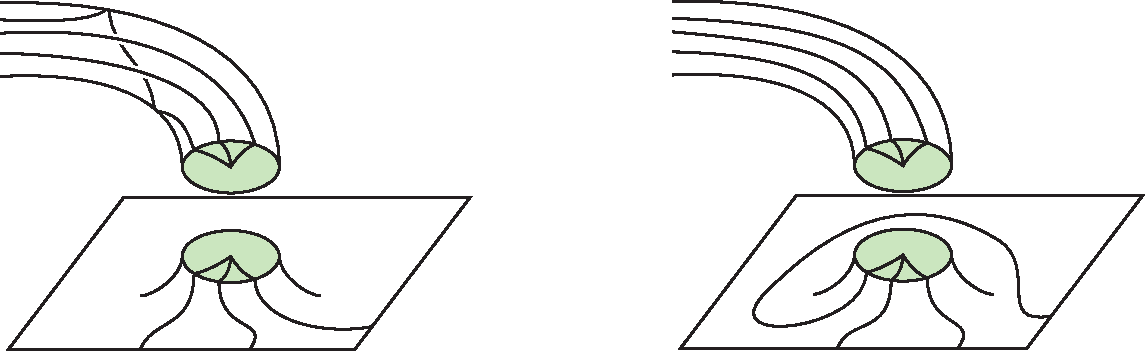
\includegraphics[scale=0.6]{OneHandlevsTetPivot.pdf} 
\caption{\label{OneHandlevsTetPivot}
 A 1-handle and its attaching region on an adjacent 0-handle (the plane denotes a section of the surface of the 0-handle).
Standardizing the 0-handle attaching regions to be ``pitchforks" requires that we either have to add pivots to the 1-handle (left, where one of the strands on the 1-handle is wrapped around the 1-handle) or to the corresponding 0-handle attaching region (right, where one strand on the 0-handle is pivoted around the attaching region). 
In \eqref{bos_tv_sum_std} we choose to include the pivots within 1-handles.}
\end{centering} 
\end{figure} 

\medskip

These standardizations also serve to make the original state sum \eqref{bos_tv_sum} more uniform.
We can now write
\be \label{bos_tv_sum_std}
	Z(M) = \sum_{\beta\in\mcl(\mch)}
		\prod_{c\in\mch_3} \mcd^{-2}
		\prod_{f\in\mch_2} d(f, \beta)
		\prod_{e\in\mch_1} \Theta(P_e, \beta)^{-1}
		\prod_{v\in\mch_0} \text{Tet}(v, \beta) .
\ee
Here $\Theta(P_e, \beta)$ is a standard pairing as in \eqref{reflection_pairing_defn}, but modified by the pivot isomorphism $P_e$.
The weight $\text{Tet}(v, \beta)$ is a standard tetrahedral symbol (though there are still variants which depend on
the orientations of the edges of the tetrahedron).
The point is that we have now written the state sum for an arbitrary 3-manifold in terms of a finite number
of standard weights.



%%%%%%%%%%%%%%%%%%%%%
\subsection{The fermionic state sum}
%%%%%%%%%%%%%%%%%%%%%


%%%%%%%%%%%%%%%%%%%%%%%%%%%%%
\subsubsection{Definition of the fermionic state sum}
%%%%%%%%%%%%%%%%%%%%%%%%%%%%%

We now extend the bosonic state sum to the fermionic case. 
We start with two pieces of data: a super pivotal fusion category $\spc$, and a spin
3-manifold $M$ possessing a cell decomposition with orientations of 1- and 2-cells.
The fermionic version of the state sum is similar to the bosonic version:
\begin{align}
\label{fermionic_tv_sum}
	Z(M) = \sum_{\beta\in\mcl(\mch)}(-1)^{\kappa_\beta}
		\prod_{c\in\mch_3} \mcd^{-2}
		\prod_{f\in\mch_2} \frac{d(f, \beta)}{n(f,\beta)}
		\prod_{e\in\mch_1}  \widetilde \Theta(e, \beta)^{-1}
		\prod_{v\in\mch_0} \text{Link}(v, \beta) .
\end{align}
The fermionic version of the state sum differs from the bosonic version in the following ways:
\begin{itemize} 
\item 
The the string nets corresponding to the 0- and 1-handle weights require a sign-ordering of their string net vertices. 
This in turn requires that the partition function is weighted by a Koszul sign $(-1)^{\kappa_\beta}$
which measures the difference between the global sign ordering coming from the 1-handles and the global sign ordering coming from the 0-handles.
\item The weights assigned to the 2-handles need to be properly normalized, 
resulting in a factor of $n(f,\beta) = \dim \End(a)$ if $a$ is the simple object labeling the core of the attaching annulus for the 2-handle $f$ by $\beta$.
\item The spin structure on $M$ determines how the basis elements which make up the labeling $\beta$ are inserted into
the graphs $\text{Link}(v)$.
\end{itemize} 
As in the previous section, we will now explain 
the factors appearing in \eqref{fermionic_tv_sum}. 

As before, we use the 2-cell orientations to define an oriented graph (unlabeled string net) on the boundary of each 0-, 1- and 2-handle.
String net graphs are assigned to the $k$-handles in the same way as in the bosonic case. 
The set of all labelings $\mcl(\mch)$ is defined as the product over all 1-handles $e$ of the basis sets $B(e)$.
For a fixed labeling $\beta \in \mcl(\mch)$, the weights are determined as follows.

The 2-handle weight $d(f, \beta)$ is defined in the same way as before. 
However we now divide by the factor $n(f, \beta) = n_a = \dim\End(a)$,
where $a$ the the simple object labeling the boundary of the core of the 2-handle.
This factor is necessary because the norm-square of the $a$-labeled loop is $n_a$.

The 1-handle weights are determined by the bilinear pairings given by each 1-handle $e$. 
When evaluating the graph on the boundary of $e$, we choose the Koszul ordering which puts the terminal vertex
immediately before the initial vertex in the ordering (similar to the convention in \eqref{reflection_pairing_defn}).

For each 0-handle $v$, $\text{Link}(v,\beta)$ is defined in the same way as in the bosonic case:
we evaluate a string net determined by the 1- and 2-handles incident on $v$ and the labeling $\beta$.
There are two subtleties here.
First, when mapping a vertex label $\mu$ from the initial (terminal) end of a 1-handle to the 0-handle adjacent to the terminal (initial) end of the 1-handle, 
we must employ the attaching map which connects the terminal (initial) end of the 1-handle to the 0-handle.
This attaching map is a spin diffeomorphism, 
and changing the attaching map by a spin flip changes the sign
of the label on the 0-handle by $(-1)^{|\mu|}$.
It is here (and only here) that the state sum is sensitive to the spin structure on $M$.
The second subtlety concerns Koszul orderings.
In order (pun noticed but not intended)
to evaluate the string net on the boundary of the 0-handle, we must choose an (arbitrary) ordering
of the string net vertices of the graph on the boundary of the 0-handle.
Thus the evaluation $\text{Link}(v, \beta)$ is arbitrary up to a sign.
However, we will see that a change of Koszul ordering which changes the sign of $\text{Link}(v, \beta)$ also produces a compensating
change in the factor $(-1)^{\kappa_\beta}$, and so the overall state sum is well defined.

\begin{figure} 
\centering
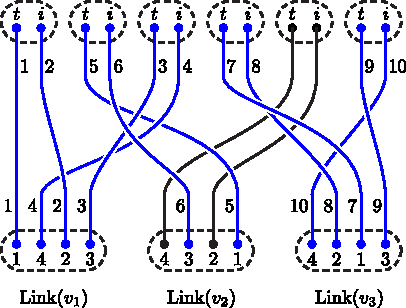
\includegraphics{KoszulFig.pdf} 
\caption{\label{KoszulFig} 
An example of how to compute the Koszul sign $(-1)^{\kappa_\beta}$ diagrammatically  
for a graph consisting of three 0-handles and six 1-handles. 
The lower dashed regions represent the 0-handles, while the upper dashed regions 
represent the 1-handles (with initial and terminal ends marked as $i$ and $t$, respectively). 
The Koszul orderings indicated by the numbers are explained in the text, and 
$\kappa_\beta$ is given by the number of crossings of the blue strands (in this example, 
$(-1)^{\kappa_\beta}=-1$).
}
\end{figure}


The Koszul sign $(-1)^{\kappa_\beta}$ is defined as follows.
Consider, for fixed $\beta$, the tensor product of the all the super vector spaces
associated to the attaching disks on all the 0-handles.
If there are $k$ 1-handles, then there are $2k$ tensor factors in this tensor product, one 
for each 1-handle end. 
We will compare two different orderings of the tensor factors.
In the first ordering, we place each terminal disk immediately before each initial disk in the ordering.
Such an ordering is well-defined up to even permutations.
In the second ordering, 
we choose a global ordering of the 0-handles and then
use the above choices of local ordering for the factors associated to
each 0-handle.
This is again well-defined up to even permutations, since each 0-handle graph evaluates to zero when the total
parity at that 0-handle is odd.
(It depends on the choice of local orderings but not on the choice of global ordering of the 0-handles.)
We then define $(-1)^{\kappa_\beta}$ to be Koszul sign relating these two orderings. 

\medskip

We now describe a convenient way to compute $(-1)^{\kappa_\beta}$ graphically, with an 
example shown in Figure \ref{KoszulFig} for a graph consisting of six 1-handles 
(upper dashed regions) and 3 0-handles $v_1,v_2,v_3$ (lower dashed regions). 
Each 0-handle has four 1-handle attaching regions, which are indicated by the lower small dots and 
which possess a local ordering relative to one another (indicated by the numbers within the lower dashed regions). 
Each attaching region can either be even (black) or odd (blue). 
If it is odd, we assign a Koszul ordering to the attaching
region, consistent with the local ordering at the 0-handle.
This ordering is indicated by the numbers appearing just outside the lower dashed regions.

Each 1-handle either has two even ends or two odd ends: if it has two odd ends, we assign an ordering 
to the ends by placing the terminal end immediately before the initial end in the ordering. This ordering
is denoted by the top row of numbers below the 1-handles in Figure \ref{KoszulFig}. 

To evaluate $(-1)^{\kappa_\beta}$, we draw a fermion line connecting each odd 0-handle attaching region
with Koszul order $k$ to the respective 1-handle end with Koszul order $k$. $(-1)^{\kappa_\beta}$ is then 
simply $(-1)^{n_c}$, where $n_c$ is the number of crossing between fermion lines in the resulting diagram. 
In the example of Figure \ref{KoszulFig} we have $n_c=11$, and so $(-1)^{\kappa_\beta}=-1$. 

\medskip

The case of non-empty $\bd M$ presents one new issue not present in the bosonic version:
we must pick a Koszul ordering of the labels corresponding to string net vertices on $\bd M$.
Once this has been done, we can combine that ordering with the ordering coming from the 1-handles.
The Koszul sign $(-1)^{\kappa_\beta}$ is now defined to be the sign arising from comparing 
the 0-handle ordering with the combined $\bd M$ and 1-handle ordering.


%%%%%%%%%%%%%%%%%%
\subsubsection{The fermionic state sum as a tensor network}
%%%%%%%%%%%%%%%%%%

We now turn to the task of reinterpreting \eqref{fermionic_tv_sum} as a tensor network.

\medskip

We incorporate the factors of $d(f, \beta)/n(f,\beta)$ and $\mcd^{-2}$ into the 0-handle 
weights 
in the same way as in the bosonic case. 
As in the bosonic case we denote the dressed 0-handle weights by $\widetilde{\rm Link}(v,\beta)$.
We define the vertex tensor in a similar fashion to \eqref{vertex_tensor}. 
Let $e_1, \cdots, e_k$ be the 1-handles adjacent to the 0-handle $v$ with the same ordering as the vertices of the graph $\text{Link}(v)$.
Let $V_i$ be defined in the same way as \eqref{0_handleVectorspaces} (with the modification that $V_i$ is a super vector space).
We define 
\begin{align} \label{Tv_defn}
T_v  \in V_1^* \tp \cdots \tp V_k^*
\end{align}
by 
\begin{align}
T_v(w_1 \tp \cdots \tp w_k) = \widetilde{\text{Link}}(v, w_1 \tp \cdots \tp w_k)
\end{align} 
where $w_i \in V_i$.
In words, $T_v$ evaluates the string-net graph determined by $\text{Link}(v)$ with the ordered vertices labeled by $w_1, \cdots, w_k$ (in the same order), and multiplied by the appropriate factors of $d(f,\beta)/n(f,\beta)$ and $\mcd^{-2}$.

As in the bosonic case, the partition function 
is computed as a trace of the $T_v$ tensors:
\be \label{fermion_Z_as_tr} Z(M) = \tr \left(\bigotimes_{v\in \mch_0} T_v\right).\ee
where the $\tr$ denotes contracting dual indices.
In practice, to perform the trace, we require that the pair of vectors to be contracted be adjacent in the Koszul ordering (with terminal preceding initial). 
To make the pair of vectors adjacent in the Koszul ordering we need to apply a number of Koszul isomorphisms. 
After contracting all vectors we pick up the appropriate factor of $(-1)^{\kappa_\beta}$. 
Again, $Z(M)$
is independent of the way we assign factors of $d(f,\beta)/n(f,\beta)$ and $\mcd^{-2}$ to the 
vertex tensors. 

If $\bd M$ is non-empty, we again follow the bosonic prescription in \eqref{trace_pM_nonempty} 
to obtain $Z(M) = \tr \left( \bigotimes_{v\in \mch_0} T_v \right) \in W_1^*\tp\cdots\tp W_n^*$, where 
$W_1, \ldots, W_n$ are the vector spaces associated to the boundary 0-cells and we 
are implicitly making use of the undordered tensor product. When using $Z(M)$ to compute 
amplitudes of different string-net boundary conditions, care must be taken when performing the 
tensor contraction on ordered representatives because of Koszul sign issues. 



%%%%%%%%%%%%%%%%%%%% 
\subsubsection{Fermionic standardization procedures} \label{fermionic_standardization}
%%%%%%%%%%%%%%%%%%%%

As in the bosonic case, we can standardize the tensor network by
choosing a generic cell decomposition (dual to a triangulation)
and ``pitchforkizing" all trivalent vertices which appear on the boundaries of 0-handles.
Note that in this fermionic setting, pitchforkizing includes choosing a spin framing at each trivalent vertex.
This standardization procedure results in string net vertices on 0-handles which are standardized independently of their partners at the opposite
ends of the 1-handles: 
the form of a given trivalent vertex at the initial edge of a 1-handle $e$
and the form of the associated vertex on the terminal edge of the 1-handle may be related by a pivot operation.
Properly accounting for this requires inserting pivot operators $P_e=P^{l_e}$ into the 
1-handles, as in \eqref{horshoe_resln}. 
Rather than tacking the spin-structure signs onto the 0-handle weights 
we incorporate them into the pivots.
Indeed, we now have $P_e^3=(-1)^F$, so that $l_e$ is 
valued in $\zz_6$ as opposed to $\zz_3$.
(Alternatively, we could keep $l_e \in \zz_3$  but insert $(-1)^{F} \cdot P^{l_e}$ where appropriate.)
Note that the spin structure of the underlying 3-manifold is encoded in the edge pivots $P_e$ (and the standardized 0-handles).

The standard tetrahedral string net on each 0-handle must of course incorporate a Koszul ordering in the fermionic case: 
\begin{align} 
	T_v(\alpha \tp \beta \tp \gamma \tp \delta) = {\rm Tet}(v,\alpha \tp \beta \tp \gamma \tp \delta) = \Tetrahedron.
\end{align}
Note that there are still multiple versions of the standardized tetrahedral weights ${\rm Tet}$ differing by choices of the edge orientations.
The fermionic analogue of \eqref{bos_tv_sum_std} can now be written:
\begin{align}
\label{ferm_tv_sum_std}
	Z(M) = \sum_{\beta\in\mcl(\mch)}(-1)^{\kappa_\beta}
		\prod_{c\in\mch_3} \mcd^{-2}
		\prod_{f\in\mch_2} \frac{d(f, \beta)}{n(f,\beta)}
		\prod_{e\in\mch_1}  \Theta(P_e, \beta)^{-1}
		\prod_{v\in\mch_0} \text{Tet}(v, \beta) .
\end{align}
Again, $\Theta(P_e, \beta)$ is a standard pairing as in \eqref{reflection_pairing_defn} but modified by the pivot isomorphism $P_e = P^{l_e}$.


%%%%%%%%%%%%%%%%%%%%%%%%%%%%%%%%%%%
\subsection{The shadow world and ground state wave functions}\label{shadowworld}
%%%%%%%%%%%%%%%%%%%%%%%%%%%%%%%%%%%

In this subsection we construct a state sum and corresponding tensor network that produces the ground state wave function of the 
Hamiltonian defined in Section \ref{Super_pivotal_Hamiltonian}.
In a nutshell, the idea is to apply the general tensor network construction of the previous subsection to the spin 3-manifold
$\Sigma\times I$, where $\Sigma$ is the spin surface which hosts the Hamiltonian.

Recall that the big Hilbert space for the Hamiltonian defined on a cell decomposition $\mcg$ is
\begin{align} \label{bhs_redef}
	\mch_\mcg =\bigotimes_{v \in \mcv} \mch_v,
\end{align}
where $\mch_v $ is defined to be $\bigoplus_{a,b,c} V^{abc}$ if all edges point away from the vertex, 
with similar definitions of $\mch_v$ in the case of other edge orientation arrangements.
If a basis vector of $\mch_\mcg$ satisfies edge label compatibility for all adjacent pairs of vertices
(equivalently, if the basis vector lies in the ground state of the vertex term of the Hamiltonian),
then it can be interpreted as defining a string net on $\Sigma$.
A wave function (not ``the" wave function unless the ground state is 1-dimensional) $\Psi$ assigns a weight $\Psi(w)$ to each such basis vector $w$, 
in such a way that if $\sum_i c_i w_i$ is equal to zero in $A(\Sigma)$, then $\sum_i c_i \Psi(w_i) = 0$.
For basis vectors $w$ which violate edge label compatibility, we have $\Psi(w) = 0$.

Given a string net $g$ on $\Sigma$, we can define a wave function $\Psi_g$ via
\be  \label{wfg-def}
	\Psi_g(w) = Z(\Sigma\times I)(\bar g \cup w) .
\ee
In other words, we evaluate the path integral $Z(\Sigma\times I)$ with boundary condition $\bar g$ on $\Sigma\times\{0\} \cong -\Sigma$
and boundary condition $w$ on $\Sigma\times\{1\} \cong \Sigma$.
(Recall that $\bar g$ is the reflected version of the string net $g$ on the orientation-reversed surface $-\Sigma$.)
Note that as $g$ runs through a basis of $A(\Sigma)$, $\Psi_g$ runs through a basis of the wave functions for the ground state of the Hamiltonian.
Our task now reduces to using the techniques of the previous subsection to construct a tensor network which evaluates the RHS of \eqref{wfg-def}.

\medskip

First we must specify a handle decomposition of $\Sigma\times I$.
Let $G'$ be the 1-skeleton of the cell decomposition of $\Sigma$ associated with $\mch_\mcg$, and let $G''$ be the 1-skeleton of the
cell decomposition of $\Sigma$ underlying the input string net $g$.
(In practice, $G'$ will be as fine a lattice as our computer can handle, while $G''$ will be as simple as possible
subject to the constraint that $g$ can represent a basis of $A(\Sigma)$.)
We stipulate that $G'$ and $G''$ are transverse (i.e., only their 1-cells intersect, and all the intersections are transverse), and are each dual to a triangulation, so that their vertices are all 3-valent.
We define the cell decomposition $G$ to be the union of $G'$ and $G''$.
The graph $G$ has three types of vertices: vertices of $G'$,
vertices of $G''$, and vertices corresponding to the points of $G'\cap G''$ which
are 4-valent; see Figure~\ref{slab_decomp}.

\begin{figure}
\begin{align}
\nonumber
\vcenter{
\xymatrix @!0 @M=2mm @R=20mm @C=50mm{
G'' & G' & G = G' \cup G'' \\
\GraphGprimeprime&\GraphGprime& \GraphG
	}}
\end{align}
\caption{\label{slab_decomp}
The cell decompositions described in the text. $G''$ (left) is the cell 
decomposition on which the input string-net state is defined, and $G'$ (center) is the decomposition on 
which the Hamiltonian acts. The union $G=G'\cup G''$ (right) is the cell decomposition we use to 
construct the ground state wavefunctions. }
\end{figure}

Our handle decomposition for $\Sigma\times I$ will be a thickened version of $G$.
We have a 0-handle for each vertex of $G$, a 1-handle for each edge of $G$, and a 2-handle for each 2-cell of the complement of $G$.
There are no 3-handles.
Figure \ref{VertexTypes} illustrates this handle decomposition, and also shows how the string nets
$v$ and $\bar g$ are situated on its boundary.


\begin{figure}
\begin{centering}
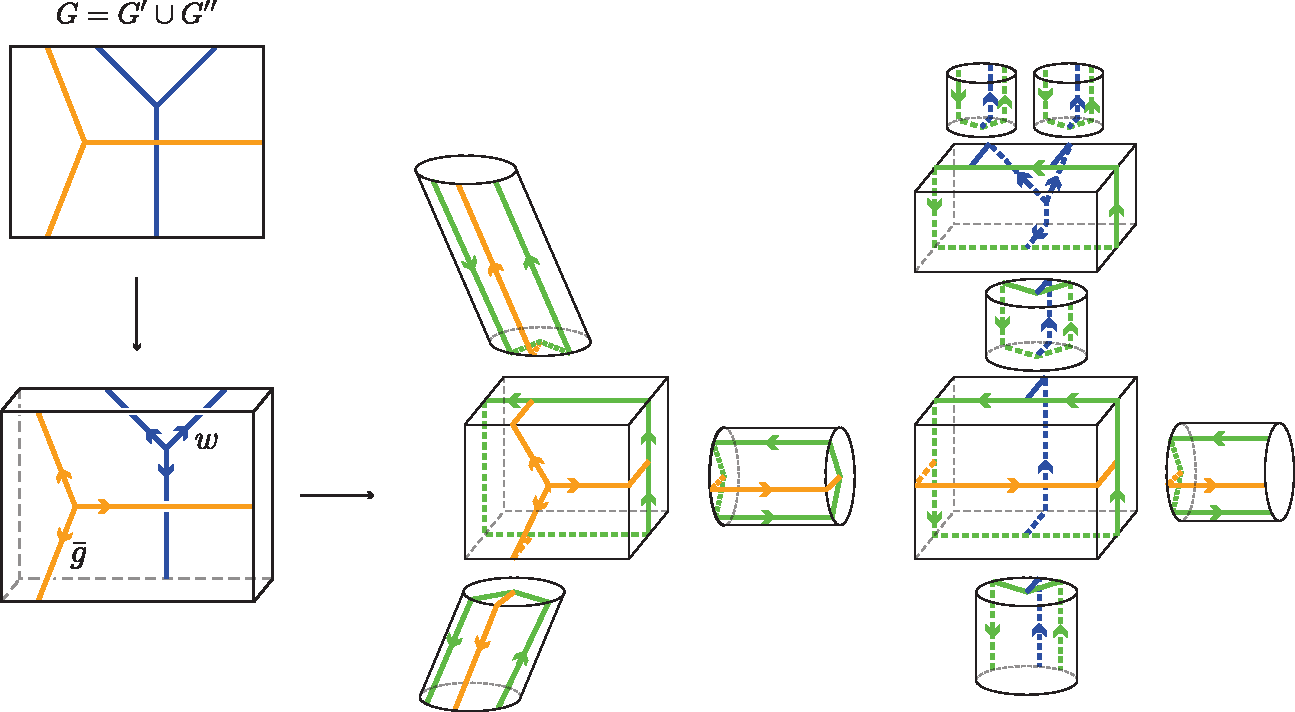
\includegraphics[scale=.7]{VertexTypes.pdf}
\caption{\label{VertexTypes}
An example cell decomposition on $\Sigma \times I$. 
In the upper left figure, we show the cell decomposition $G$ for a given simple choice of $G'$ (blue) and $G''$ (orange). 
In the lower left figure, we include the ``time direction'' in the picture, which thickens it into a box with boundary conditions 
set by $\bar g$ on the initial boundary $\Sigma \times \{0\}$ and boundary conditions set by $w$ on the terminal boundary $\Sigma \times \{1\}$. 
The right figure shows the full handle decomposition for this setup. Each box shows a 0-handle in the composite cell decomposition $G$, 
while each cylinder shows a 1-handle. The green lines denote string nets in the interior of $\Sigma \times I$, which are not fixed 
by either of the boundary conditions $\bar g, v$.
}
\end{centering}
\end{figure}


The next step is to standardize the string nets on the boundary of each 0-handle, by following the procedures outlined in Sections \ref{bosonic_standardization} and \ref{fermionic_standardization}.
This is illustrated in Figure \ref{StandardizedSlabTensorsprime} for the three different types of 0-handle in our handle decomposition $G$ (one of each type of 0-handle is shown in the rightmost picture of Figure \ref{VertexTypes}).
Note that our conditions on the handle decompositions $G',G''$ ensure that all three types of 0-handle string nets are tetrahedral.

\medskip

We are now in a position to apply the state sum and tensor network constructions of the previous subsection.
The state sum turns out to be a version of the ``shadow world" state sum of \cite{kirillow1989,turaev2016quantum}. 
In other words, the shadow world state sum is a special case of the Turaev-Viro state sum.
If we fix the (labeled) string net $\bar g$ at the outset, the tensor network has an output corresponding to \eqref{bhs_redef}.

\begin{figure}
\begin{center}
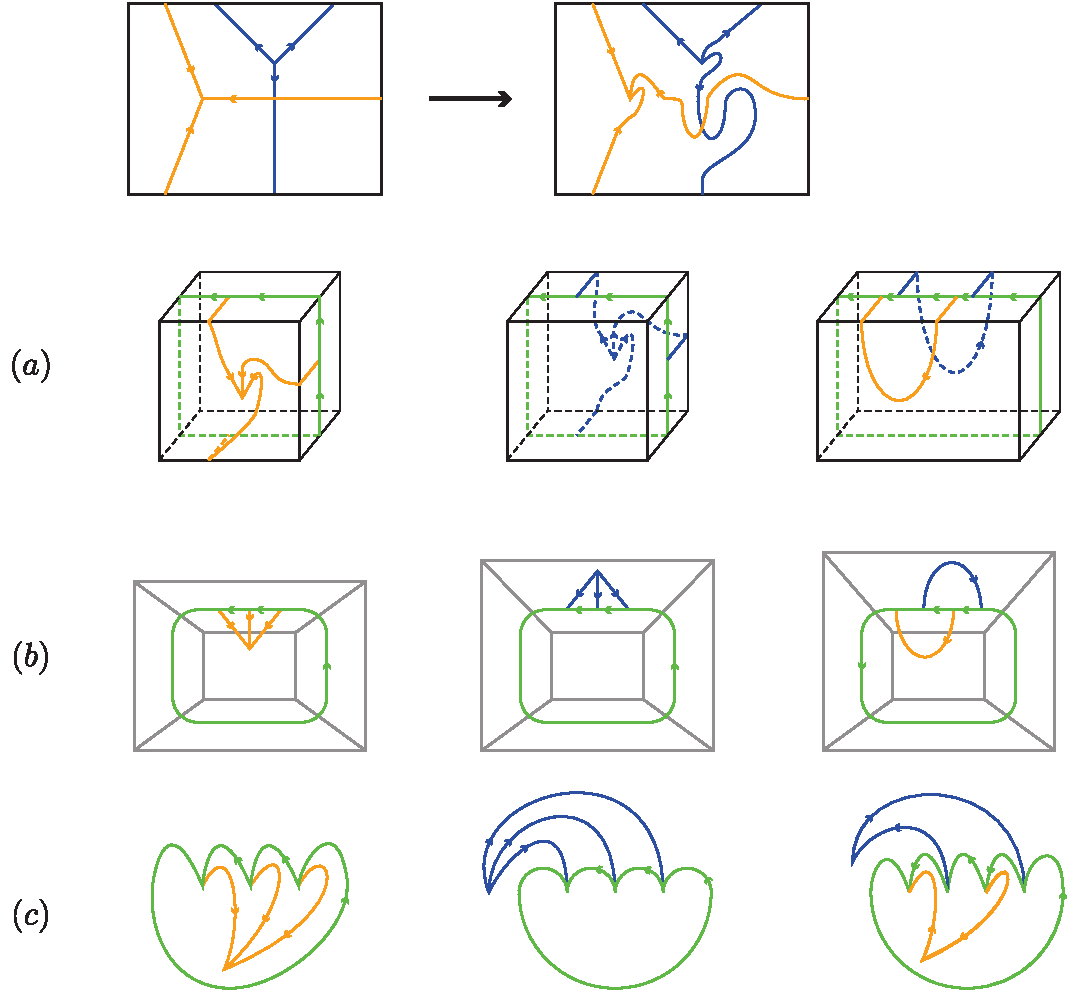
\includegraphics[scale=0.6]{CurGraphStandardization.pdf}
\caption{\label{StandardizedSlabTensorsprime} \label{StandardizedSlabTensors}
The different types of 0-handles that appear in the cell decomposition of $G$. 
The top picture shows how a simple cell decomposition is standardized by putting 
each of the trivalent vertices in pitchfork form. 
In row (a) we show the three different types of standardized 0-cells that can appear in $G$. The cubes are drawn so that the 0-cells are located in their centers. 
Orange (blue) lines represent 1-handles in $G''$ ($G'$), and 
green lines represent intersections of 2-cells in $G$ with the cube. 
In row (b) we show the standardized string nets projected into the plane, and in  
row (c) we finish the standardization of the diagrams by making each trivalent vertex a pitchfork. The appropriate 0-cell 
tensors are found by evaluation of these diagrams. 
}
\end{center}
\end{figure}

To compute the tensor network, we just need to know how to assign tensors to the 0-handles in $G$. 
This is done by computing evaluations of tetrahedral string-net diagrams, as in previous sections. 
Explicitly, for a 0-cell $v$ of $G$ consisting of three 1-cells of $G'$ (middle column of row (a) of Figure \ref{StandardizedSlabTensorsprime}), 
we assign the tensor $T_v$ as follows: 
\begin{align}
\Tensora \; \ra T_v(\mu_0 \tp s_1 \tp s_2 \tp s_3) &= \;  \Tensorcc\,,
\end{align}
In the diagrams, the green letters $A,B,C$ denote the labels of the 2-cells in the ``interior'' of the cell decomposition on $\Sigma \times I$ (those drawn in green in Figure \ref{VertexTypes}), which will 
be summed over when computing the amplitude $Z(\Sigma\times I)(\bar g \cup v)$. The labels of 
the blue lines are fixed, and are determined by the labels of the 1-cells 
in the string-net graph $v$ on $\Sigma \times \{1\}$. 

Tensors for the other types of 0-cells in $G$ are determined similarly. For the type of 
0-cell in the left column of row (a) in Figure \ref{StandardizedSlabTensorsprime} involving three 1-handles from $G''$, we assign the tensor
\begin{align}
\Tensorc \;\ra  T_v(\nu_0 \tp s_1 \tp s_2 \tp s_3) &= \; \Tensoraa\,, \\
\end{align}
where the labels of the orange lines are fixed by the input string-net state $\bar g$.
Similarly, for the type of 0-cell in the right column (involving the intersection of 1-handles in $G'$ and $G''$) we assign the tensor
\begin{align}
\Tensorb \; \ra T_v(s_0 \tp s_1 \tp s_2 \tp s_3) &= \;  \Tensorbb\,, \\
\end{align}
which corresponds to a string operator. 

Now that we know how to assign tensors to each 0-handle, we can construct the partition function $Z(\Sigma \times I)(\bar g \cup v)$ in the same way as in previous sections, namely by performing a tensor contraction over $\bigotimes_{v\in \mch_0}T_v$, 
where the tensor product runs over all 0-cells of $G$.
(The evaluation of this tensor contraction involves the same 
treatment of Koszul signs and 1-handle pivots as the fermionic state sum discussed in the previous section.)

\medskip

Instead of fixing a particular input string net $g$, we can put $g$ and $v$ on more equal footing by constructing
a tensor network which computes an operator from $\mch_{G''}$ to $\mch_{G'}$, where $\mch_{G''}$ and $\mch_{G'}$ are versions of \eqref{bhs_redef} corresponding to the vertices of $g$ and $v$, respectively. 
In particular, we can take $G''$ to be isotopic\footnote{
We can't take $G'' = G'$ because we require that $G'$ and $G''$ be transverse.}
to $G'$ and compute a projection from the big Hilbert space to itself.
This projection is, of course, the projection onto the ground state of the Hamiltonian of Section \ref{Super_pivotal_Hamiltonian}.

There is one small technical hurdle to overcome before constructing this operator.
Previously we adopted the convention that boundaries of 3-manifolds are contained in the 2-skeletons of cell decompositions 
corresponding to handle decompositions.
This is convenient for many purposes, but if we want to glue 3-manifolds along their boundaries (and perform analogous operations with
tensor networks), then it would have been more convenient to take the boundaries to be transverse to the cell decompositions.
In practice, this means that we must assign some additional factors of $\mcd^{-2}$ and $d_a/n_a$ to our 0-handle tensors (as described above \eqref{0_handleVectorspaces}), corresponding to
3- and 2-cells which straddle the surface along which we are gluing 3-manifolds.
Specifically, for each 2-cell of $G''$ we choose an adjacent 0-cell and assign a factor of $\mcd^{-2}$ to the corresponding 0-handle tensor,
and to each 1-cell of $G''$ we choose an adjacent 0-cell and assign a factor of $d_a/n_a$ to the corresponding 0-handle tensor.
These 2- and 1-cells in $\Sigma$ correspond to the 3- and 2-cells which straddle the gluing surface when we glue two copies
of $\Sigma\times I$ together.

Let $H$ denote the resulting tensor network operator. 
The fact that $(\Sigma\times I) \cup (\Sigma\times I) \cong \Sigma\times I$ implies that
$H\circ H = H$.
The fact that $\Sigma\times I \cong -(\Sigma\times I)$ 
(via a homeomorphism which is the identity on the $\Sigma$ factor and reverses the $I$ factor)
implies that $H$ is self-adjoint
(see the end of Section \ref{reflection_ss}).

